\documentclass{beamer}
\usepackage{graphicx}
\usepackage{beamerthemesplit}
\usepackage{amsmath, amssymb, amsthm}
\usepackage{color}
\usepackage{mathtools}
\usetheme{Warsaw}
\usepackage{geometry}
\usepackage{epstopdf}
\usepackage{wrapfig}
\usepackage[latin1]{inputenc}
\usepackage{tikz}
\usetikzlibrary{shapes,arrows}
\usepackage{caption}
\usepackage{algorithm}
\usepackage{algorithmic}
\usepackage{longtable}
\usepackage{bbm}
\usepackage{relsize}
\usepackage{enumerate}
\usepackage{bm}
\usepackage{amsfonts}
\usepackage{graphicx}
\captionsetup[figure]{labelformat=empty}



\newcommand{\E}{\mathbb{E}}
\newcommand{\KG}{\mathrm{KG}}
\newcommand{\KGs}{\mathrm{KG}}
\newcommand{\KGp}{\mathrm{KG}^2}
\newcommand{\nuKGp}{\nu^{KG2}}
\newcommand{\zap}[1]{}
\newcommand{\twovec}[2]{\left( \begin{array}{c}#1\\ #2\end{array} \right)}
\newcommand{\twomatrix}[4]{\left(\begin{array}{cc}#1&#2\\#3&#4\end{array}\right)}
\newcommand{\Prob}{\mathbb{P}} % probability measure
\newcommand{\e}[1]{\left\{#1\right\}}
\newcommand{\s}[1]{\left[ #1 \right]}
\newcommand{\length}{\mathrm{length}}
\newcommand{\Ytilde}{\widetilde{Y}}
\newcommand{\Fn}{\mathcal{F}_n}
\newcommand{\Ncal}{\mathcal{N}}
\newcommand{\Var}{\mathrm{Var}}
\newcommand{\R}{\mathbb{R}}
\newcommand{\N}{\mathbb{N}}
\newcommand{\Z}{\mathbb{Z}}
\newcommand{\lsb}{\left[}
\newcommand{\rsb}{\right]}
\newcommand{\lp}{\left(}
\newcommand{\sigmatilde}{\tilde{\sigma}}
\newcommand{\rp}{\right)}
% \newcommand{\xvec}{{\bf x}}
% \newcommand{\Yvec}{{\bf Y}}
\newcommand{\xvec}{x}
\newcommand{\Yvec}{Y}

\newcommand{\figref}[1]{Figure~\ref{#1}}
\newcommand{\secref}[1]{\S\ref{#1}}     % NB: Still sshould write Section~\ref{ABC} at start of a sentence
\newcommand{\secrefb}[2]{\S\ref{#1}-\S\ref{#2}}

\newcommand{\omg}{\omega}
\newcommand{\Sv}{\mathbf{S}}
\newcommand{\Sb}{\mathbb{S}}
\newcommand{\Ab}{\mathbb{A}}
\newcommand{\Pb}{\mathbb{P}}
\newcommand{\Rb}{\mathbb{R}}
\newcommand{\Eb}{\mathbb{E}}
\newcommand{\av}{\mathbf{a}}
\newcommand{\bv}{\mathbf{b}}
\newcommand{\Nv}{\mathbf{N}}
%\newcommand{\cv}{\mathbf{c}}
\newcommand{\cv}{c}
%\newcommand{\dv}{\mathbf{d}}
\newcommand{\dv}{d}
\newcommand{\muv}{\pmb{\mu}}
\newcommand{\betav}{\pmb{\beta}}
%\newcommand{\thetav}{\pmb{\theta}}
\newcommand{\thetav}{\theta}
\newcommand{\lambdav}{\pmb{\lambda}}
\newcommand{\alphav}{\pmb{\alpha}}
%\newcommand{\thetav}{\theta}
\newcommand{\NoGa}{\mathcal{NG}}
\newcommand{\zv}{\mathbf{z}}
\newcommand{\wv}{\mathbf{w}}
\newcommand{\ev}{\mathbf{e}}
\newcommand{\allpv}{\pmb{\allp}}
\newcommand{\Pv}{\mathbf{P}}
\newcommand{\Fcal}{\mathbf{F}}
%------------MACROS for entire/sub problems---------
\newcommand{\allp}{\pmb{\pi}}
\newcommand{\allpset}{\mathbf{\Pi}}
\newcommand{\allstates}{\mathbb{S}^K}
\newcommand{\allstate}{\mathbf{s}}
\newcommand{\allstater}{\mathbf{S}}
\newcommand{\allactions}{\mathbb{A}^K}
\newcommand{\allaction}{\av}
\newcommand{\allar}{\mathbf{A}}
\newcommand{\allpr}{\mathbb{P}}
\newcommand{\allr}{R}

\newcommand{\subp}{\pi}
\newcommand{\subpset}{\Pi}
\newcommand{\subr}{r}
\newcommand{\substates}{\mathbb{S}}
\newcommand{\substater}{S}
\newcommand{\substate}{s}
\newcommand{\subactions}{\mathbb{A}}
\newcommand{\subar}{A}
\newcommand{\subpr}{P}
\newcommand{\subaction}{a}

\begin{document}
\title{Sequential Resource Allocation Under Uncertainty: An Index Policy Approach}
\author{Weici Hu\\
Adviser: Peter Frazier\\
\hspace{1mm}\\
Cornell ORIE}
\begin{frame}
   \maketitle
\end{frame}
%%%%%%%%%%%%%%%%%%%%%%%%%%%%%%%%%%%%%%%%%%%%%%%%

%%%%%%%%%%%%%%%%%%%%%%%%%%%%%%%%%%%%%%%%%%%%%%%%
\begin{frame}
\frametitle{Problem Setup}
We consider an MDP $(\allstates,\allactions,\allpr^{\cdot},\allr)$ that consists of K identical sub-processes $(\substates,\subactions,\subpr^{\cdot},\subr)$, specifically,
\begin{itemize}
\item Time horizon $T<\infty$.
\item State space $\allstates$ is the cross-product of $K$ $\substates$. $\substates$ is assumed finite.
\item Action space $\allactions$ is the cross-product of $K$ $\subactions$. $\subactions=\{0,1\}$.
\item Reward $\allr_t(\allstate,\allaction) = \sum_{x=1}^K \subr_t(\substate_x,\subaction_x)$, $1\leq t\leq T$, is additive of the reward of individual sub-processes.
\item Transition probability $\allpr^{\allaction}(\allstate',\allstate) = \prod_{x=1}^{K}\subpr^{\subaction_x}(\substate'_x,\substate_x)$.
\end{itemize}
\end{frame}
%%%%%%%%%%%%%%%%%%%%%%%%%%%%%%%%%%%%%%%%%%%%%%%%

%%%%%%%%%%%%%%%%%%%%%%%%%%%%%%%%%%%%%%%%%%%%%%%%
\begin{frame}
\frametitle{Problem Setup Con't}
\begin{itemize}
\item A Markov policy $\allp:\allstates\times \allactions \times \{1,...,T\} \rightarrow [0,1]$, with $\allp(\allstate,\allaction,t) = P(\allaction|\allstater_t=\allstate)$ (Our decision).\\ We require $\sum_{\allaction\in\allactions}\allp(\allstate,\allaction,t)=1$.
$\forall \allstate\in\allstates, \forall 1\leq t\leq T$.
\item Objective
\begin{equation}\label{prime}
\begin{aligned}
& \underset{\allp\in\allpset}{\text{maximize}}
& & \mathbb{E}^{\allp}\left[\sum_{t=1}^{T}\allr_t\big(\allstater_t,\allar_t\big)\right] \\
& \text{subject to}
& & P^{\allp}(|\allar_t|=m_t)=1, \hspace{3mm}\forall 1\leq t\leq T .
\end{aligned}
\end{equation}
\end{itemize}
\end{frame}
%%%%%%%%%%%%%%%%%%%%%%%%%%%%%%%%%%%%%%%%%%%%%%%%

%%%%%%%%%%%%%%%%%%%%%%%%%%%%%%%%%%%%%%%%%%%%%%%%
\begin{frame}
\frametitle{Difficulty: Optimal solutions are computationally infeasible}
Optimal solutions of \eqref{prime} can be obtained with Bellman optimality equations.

\vspace{0.5cm}
But it requires $O(|\substates|^K|\subactions|^KT)$ time complexity and $O(|\substates|^K|\subactions|^KT)$ storage complexity.

\vspace{0.5cm}
The complexity grow exponentially with the number of sub-processes $K$, and becomes computationally infeasible for large $K$.
\end{frame}
%%%%%%%%%%%%%%%%%%%%%%%%%%%%%%%%%%%%%%%%%%%%%%%%

%%%%%%%%%%%%%%%%%%%%%%%%%%%%%%%%%%%%%%%%%%%%%%%%
\begin{frame}
\frametitle{Past attempts}
\end{frame}
%%%%%%%%%%%%%%%%%%%%%%%%%%%%%%%%%%%%%%%%%%%%%%%%

%%%%%%%%%%%%%%%%%%%%%%%%%%%%%%%%%%%%%%%%%%%%%%%%
\begin{frame}
\frametitle{Pre-computations: 1. Optimal Lagrange Multiplier of \eqref{prime}}
Relax the original problem \eqref{prime} to
\begin{equation}\label{prime2}
\begin{aligned}
& \underset{\allp\in\allpset}{\text{maximize}}
& & \mathbb{E}^{\allp}\left[\sum_{t=1}^{T}\allr_t\big(\allstater_t,\allar_t\big)\right] \\
& \text{subject to}
& & \mathbb{E}^{\allp}(|\allar_t|)=m_t, \hspace{3mm}\forall 1\leq t\leq T .
\end{aligned}
\end{equation}
The Lagrangian relaxation of \eqref{prime2}
\begin{equation}\label{ub}
 P(\lambdav)=\max_{\allp\in \allpset}\mathbb{E}^{\allp}\left[\sum_{t=1}^{T}\allr_t\big(\allstater_t,\allar_t\big)\right]-\sum_{t=1}^T\lambda_t\left(\mathbb{E}^{\allp}[|\allar_t|]-m_t\right).
 \end{equation} 
\end{frame}
%%%%%%%%%%%%%%%%%%%%%%%%%%%%%%%%%%%%%%%%%%%%%%%%

%%%%%%%%%%%%%%%%%%%%%%%%%%%%%%%%%%%%%%%%%%%%%%%%%
\begin{frame}
\frametitle{Pre-computations: 1. Optimal Lagrange Multiplier of \eqref{prime}}
Decomposition of the Lagrangian relaxation
\begin{equation}\label{dec}
P(\lambdav)=K Q(\lambdav) + \sum_t\lambda_t m_t,
\end{equation}
where
\begin{equation}\label{dpx}
Q(\lambdav)=\max_{\subp\in \subpset}\mathbb{E}^{\subp}\left[\sum_{t=1}^{T}\subr_t(\substater_t,\subar_t)-\lambda_t \subar_t\right],
\end{equation}
is the objective function for sub-process $(\substates,\subactions,\subpr^{\cdot},\subr)$. Definition of policy $\subp$ is similar to $\allp$, with  $\subp(\substate,\subaction,t) = P(\subaction|\substater_t=\substate)$.

\vspace{0.5cm}
Remark: Problem \eqref{dpx} can be solved using the Bellman recursion with complexity $O(|\substates||\subactions|T)$,  hence it is computationally feasible.
\end{frame}
%%%%%%%%%%%%%%%%%%%%%%%%%%%%%%%%%%%%%%%%%%%%%%%%%

%%%%%%%%%%%%%%%%%%%%%%%%%%%%%%%%%%%%%%%%%%%%%%%%%
\begin{frame}
\frametitle{Pre-computations: 2. Occupation Measure $\rho^*$}
Alternatively we can compute $$
\end{frame}
%%%%%%%%%%%%%%%%%%%%%%%%%%%%%%%%%%%%%%%%%%%%%%%%%

%%%%%%%%%%%%%%%%%%%%%%%%%%%%%%%%%%%%%%%%%%%%%%%%%
\begin{frame}
\frametitle{The Optimal Policy Puts Samples Where They Help Most}
%    \begin{figure}
%      \centering
%      \only<1>{\includegraphics[width=4in]{MCC2a.pdf}}
%      \only<2>{\includegraphics[width=4in]{MCC3a.pdf}}
%      \only<3>{\includegraphics[width=4in]{MCC3b.pdf}}
%    \end{figure}
\end{frame}
%%%%%%%%%%%%%%%%%%%%%%%%%%%%%%%%%%%%%%%%%%%%%%%%

%%%%%%%%%%%%%%%%%%%%%%%%%%%%%%%%%%%%%%%%%%%%%%%%%
\begin{frame}
\frametitle{Literature Review}

Related work for MCS in simulation scenario:
\begin{itemize}
\item Frequentist work: Paulson (1952) and Dunnett (1955)(one-stage procedure, normal sampling); Dudewicz and Dalal (1983), Bofinger and Lewis (1992), Damerdji and Nakayama (1996) (Two stage procedures, more general sampling distributions)
\item Similar work: Xie and Frazier (2013)(Fully sequential in a Bayesian setting)
\begin{itemize}
\item We consider a finite horizon, rather than a geometric horizon and infinite horizon.
\item We allow cost per sample to be optional.
\item We look at allocating parallel simulation resources
\end{itemize}
\end{itemize}
\end{frame}
%%%%%%%%%%%%%%%%%%%%%%%%%%%%%%%%%%%%%%%%%%%%%%%%%


%%%%%%%%%%%%%%%%%%%%%%%%%%%%%%%%%%%%%%%%%%%%%%%%%
\begin{frame}
\frametitle{Literature Review}

Related work for crowdsourcing scenario:
\begin{itemize}
\item RayKar et al(2010), Whitehill et al(2009)(static inference); Thanh et al(2013)(static budget allocation); Karger et al(2013)(dynamic assignment of tasks but require large worker budget)
\item Similar work: Chen et al(2013)(dynamic allocation under Bayesian framework with optimal policy in the form of a DP)
\begin{itemize}
\item We offer an upper bound in addition to a heuristic
\item We consider a continuous time horizon and a M/M/k queue to model the flow of workers.
\end{itemize}
\end{itemize}
\end{frame}
%%%%%%%%%%%%%%%%%%%%%%%%%%%%%%%%%%%%%%%%%%%%%%%%%

%%%%%%%%%%%%%%%%%%%%%%%%%%%%%%%%%%%%%%%%%%%%%%%%
\begin{frame}{Problem set-up for simulation scenario}

\begin{itemize}
\item $k$ alternatives
\item $m$ parallel simulating resources per time step
\item $N$ time horizon
\item $\theta_x$ is the underlying true performance of alternative $x$, $x\in\{1,...,k\}$
\item $d_x$ the known threshold for alternative $x$
\item $z_{n,x}$ is the number of simulation resources to use on alternative $x$ at time step $n$. This is our allocation decision. $\sum_x z_{n,x}\leq m$
\item After time step $N$, for each alternative $x$, we decide whether $\theta_x>d_x$ based on the past results of simulation
\item We obtain a reward $R = \sum_x R_x$. $R_x$ can be a 0-1 reward or linear reward.
\end{itemize}
{\Large \color{red} Goal:Find an allocation of simulation resources to best support the decision at time N}
\end{frame}
%%%%%%%%%%%%%%%%%%%%%%%%%%%%%%%%%%%%%%%%%%%%%%%%%%%

%%%%%%%%%%%%%%%%%%%%%%%%%%%%%%%%%%%%%%%%%%%%%%%%%%%
\begin{frame}{Problem set-up for crowdsourcing scenario}

\begin{itemize}
\item $k$ labeling tasks
\item $N$ total workers
\item $T$ time horizon
\item M/M/k queue: workers come in with rate $r$, and complete their job with rate $\mu$.
\item $\theta_x$ is the underlying likelihood for a task to have a positive label.
\item $d_x$ the known threshold for alternative $x$
\item $z_{l,x}\in \{0,1\}$ indicates whether the $l^{th}$ worker is assigned to task $x$.
\item After worker budget $N$ has been exhausted or time $T$ has been reached, for each alternative $x$, we decide whether whether the true label is positive or negative based on a 1-0 reward.
\end{itemize}
{\Large \color{red} Goal:Find an allocation of workers to best support the final decision on true labels}\end{frame}
%%%%%%%%%%%%%%%%%%%%%%%%%%%%%%%%%%%%%%%%%%%%%%%%

%%%%%%%%%%%%%%%%%%%%%%%%%%%%%%%%%%%%%%%%%%%%%%%%
\begin{frame}{We use a Bayesian approach}

Use the simulation-scenario as an example:
\begin{itemize}
\item $Y_{n,x}$ is the number of successes observed after we do $z_{n,x}$ simulations on alternative $x$ at time $n$
\[Y_{n,x}|\theta_x,z_{n,x}\sim \mathrm{Binomial}(z_{n,x},\theta_x)\]
\item We use Beta as a conjugate prior 
$\theta_x$ \[\theta_x \sim \mathrm{Beta}(\alpha_{0,x},\beta_{0,x}).\]
\begin{equation*}
  \theta_x | z_{1,x}, Y_{1,x}, \ldots, z_{n,x}, Y_{n,x} 
  \sim \mathrm{Beta}(\alpha_{n,x},\beta_{n,x}).
\end{equation*}
\end{itemize}
The Bayesian approach for the crowdsourcing scenario works in similar manner.
\end{frame}
%%%%%%%%%%%%%%%%%%%%%%%%%%%%%%%%%%%%%%%%%%%%%%%%

%%%%%%%%%%%%%%%%%%%%%%%%%%%%%%%%%%%%%%%%%%%%%%%%
\begin{frame}
\frametitle{We use a Bayesian approach}
The allocation problem under Bayesian framework is 
\begin{equation}\label{optV}
\sup_{\pi} \mathbb{E}^{\pi} \left[R\Big|\text{prior}\right]
\end{equation}
Where a policy $\pi$ is a mapping from histories onto allocations of resources with:
\begin{itemize}
\item  $\zv_n = (z_{n,1},\ldots,z_{n,k})\in \mathbb{N}^k$ satisfying \[\sum_{x=1}^k z_{n,x}\leq m\] for simulation scenario
\item $\zv_l = (z_{l,1},...,z_{l,k}) \in \mathbb{N}^k$ satisfying \[\sum_{x=1}^k z_{l,x}\leq 1\] for crowdsourcing scenario
\end{itemize}
\end{frame}
%%%%%%%%%%%%%%%%%%%%%%%%%%%%%%%%%%%%%%%%%%%%%%%%

%%%%%%%%%%%%%%%%%%%%%%%%%%%%%%%%%%%%%%%%%%%%%%%%
\begin{frame}{Dynamic Programming gives an optimal solution}
We formulate the simulation problem as a dynamic program with
\begin{itemize}
\item state at time $n$, $\Sv_n = (s_{n,1},\ldots,s_{n,k})$ = posterior parameters of all the alternatives
\item value function $V_n(\Sv_n)$ = the maximum expected total reward to be obtained from time step n onward given the current state $\Sv_n$.
\item The optimal value is $V_0(\mathbf{S}_0)$ = (\ref{optV})
\item The optimal policy $\pi^*$ is the sequence of $\zv_1^*,\ldots,\zv_N^*$ that achieves the maximum in Bellman's recursion
\end{itemize}
\end{frame}
%%%%%%%%%%%%%%%%%%%%%%%%%%%%%%%%%%%%%%%%%%%%%%%%

%%%%%%%%%%%%%%%%%%%%%%%%%%%%%%%%%%%%%%%%%%%%%%%%
\begin{frame}{Dynamic Programming gives an optimal solution}

Similarly, we formulate the crowdsourcing problem as a dynamic program.
\begin{itemize}
\item Possible transitions: a worker comes into the system; a worker completes a task and leaves the system. 
\item $\Sv_n = (\alphav,\betav,t,\mathbf{w},l)$, where $n$ denotes $n^{th}$ transition, $\alphav,\betav$ are posterior parameters, $t$ is the time the $n^{th}$ transition happens, $\mathbf{w}$ is the number of workers working on each task $x$, $l$ is the total number of workers have arrived.
\item Inter-transition time $\Delta_n \sim$ Exp$(\mu|\mathbf{w}|+r)$
\item The optimal value is $V_0(\mathbf{S}_0)$ = (\ref{optV})
\item The optimal policy $\pi^*$ is the sequence of $\zv_1^*,\ldots,\zv_N^*$ that achieves the maximum in Bellman's recursion
\end{itemize}
\end{frame}
%%%%%%%%%%%%%%%%%%%%%%%%%%%%%%%%%%%%%%%%%%%%%%%%

%%%%%%%%%%%%%%%%%%%%%%%%%%%%%%%%%%%%%%%%%%%%%%%%
\begin{frame}{Problem: Dynamic Programming is computationally infeasible}

\begin{itemize}
\item In the simulation scenario:
\begin{itemize}
\item The number of states in state space at time n is $O((mn)^k)$.
\vspace{2mm}
\item Memory scales exponentially in $k$.
\vspace{2mm}
\item Computation scales exponentially in $k$.
\vspace{2mm}
\item E.g., $m = k = 8$, at time step $N=5$, there are $2.35426*10^{12}$ states.
\vspace{2mm}
\end{itemize}
\item Even more complex in crowdsourcing scenario.
\end{itemize}
{\Large \color{blue} Curse of Dimensionality!}\\
\end{frame}
%%%%%%%%%%%%%%%%%%%%%%%%%%%%%%%%%%%%%%%%%%%%%%%%

%%%%%%%%%%%%%%%%%%%%%%%%%%%%%%%%%%%%%%%%%%%%%%%%
\begin{frame}
\frametitle{Our approach: Upper bound+heuristics}
\begin{itemize}
\item We first calculate an upper bound to the original problem.
\item We then propose an index-based heuristic policy.
\item We use the upper bound to measure the performance of the heuristic policy.
\end{itemize}
\end{frame}
%%%%%%%%%%%%%%%%%%%%%%%%%%%%%%%%%%%%%%%%%%%%%%%%

%%%%%%%%%%%%%%%%%%%%%%%%%%%%%%%%%%%%%%%%%%%%%%%%
\begin{frame}{Forming an upper bound}
%\centering
%  \includegraphics[width=0.8\textwidth]{ub_flowchart_1.png}
%%\tikzstyle{decision} = [diamond, draw, fill=blue!20, 
%%    text width=8em, text badly centered, node distance=5cm, inner sep=-10pt]
%%\tikzstyle{block} = [rectangle, draw, fill=blue!20, 
%%    text width=8em, text centered, rounded corners, minimum height=2em]
%%\tikzstyle{line} = [draw, -latex']
%%\tikzstyle{cloud} = [draw, ellipse,fill=red!20, node distance=5cm,
%%    minimum height=2em]
%% \centering 
%%\begin{tikzpicture}[node distance = 15mm, auto]
%%    % Place nodes
%%    \node [block] (init) {MCS problem};
%%   \node [cloud, right of=init] (system) {Lagrangian Relaxation};
%%    \node [block, below of=init] (identify) {relaxed problem};
%%    \node [cloud, right of=identify] (decom) {decomposition};
%%    \node [block, below of=identify] (evaluate) {$k$ single-alternative MCS problems};
%%   \node [cloud, right of=evaluate] (upp) {Computable upper bound};
%%    % Draw edges
%%    \path [line] (init) -- (system);
%%    \path [line] (system) --  (identify);
%%    \path [line] (identify) --  (decom);
%%    \path [line] (decom) -- (evaluate);
%%    \path [line] (evaluate) -- (upp);
%%\end{tikzpicture}
\end{frame}
%%%%%%%%%%%%%%%%%%%%%%%%%%%%%%%%%%%%%%%%%%%%%%%%

%%%%%%%%%%%%%%%%%%%%%%%%%%%%%%%%%%%%%%%%%%%%%%%%
\begin{frame}{Step 1 in forming an upper bound:\\Lagrangian Relaxation}

\begin{itemize}
\item Original set of feasible policies:
\[\Pi = \{\pi=(\zv_1,...,\zv_N):\sum_{x=1}^k z_{n,x}\leq m\}\]
\item Relaxed set of policies:
\[\Pi_1 = \{\pi=(\zv_1,...,\zv_N):\text{no constraint}\}\]
\item Define $V_0^{\lambdav}(\Sv_0) = \sup_{\pi\in \Pi_1}\mathbb{E}^{\pi}[R-\sum_{n=1}^N(\lambda_n(\sum_{x=1}^kz_{n,x}-m))]$
\end{itemize}
\begin{lemma}[1]
For $\lambdav\geq 0$, we have
\begin{equation*}
V_0^{\lambdav}(\Sv_0) \geq V_0(\Sv_0)
\end{equation*}
\end{lemma}

\end{frame}
%%%%%%%%%%%%%%%%%%%%%%%%%%%%%%%%%%%%%%%%%%%%%%%%

%%%%%%%%%%%%%%%%%%%%%%%%%%%%%%%%%%%%%%%%%%%%%%%%
\begin{frame}{Step 2 in forming an upper bound:\\ Decompose the relaxed DP to single-alternative DPs}
\begin{itemize}
\item Define $V_{0,x}^{\lambdav}(S_{0,x}) = \sup_{\pi^{(x)}\in \Pi^{(x)}}\mathbb{E}^{\pi^{(x)}}\left[R_x - \sum_{n=1}^{N}\lambda_nz_{n,x}\Big|S_{0,x}\right]$, $\forall x$,\\
where $\Pi^{(x)}=\{\pi^{(x)} = (z_{1,x},z_{2,x},...,z_{N,x}): z_{n,x}\leq m, \forall 1\leq n\leq N\}$
\end{itemize}
\begin{lemma}[2]
For any $\lambdav>\mathbf{0}$, let $V_{0,x}^{\lambdav}(S_{0,x})$ be the value of an single-alternative MCS problem on $x$, 
\begin{equation} \label{decom}
\footnotesize
V_{0}^{\lambdav}(\Sv_0) = \sum_{x=1}^k V_{0,x}^{\lambdav}(S_{0,x}) + m\sum_{n = 1}^{N}\lambda_{n},
\end{equation}
\end{lemma}
\begin{itemize}
\item Solving single-alternative MCS problems by dynamic programming is computationally feasible.
\end{itemize}


\end{frame}
%%%%%%%%%%%%%%%%%%%%%%%%%%%%%%%%%%%%%%%%%%%%%%%%

%%%%%%%%%%%%%%%%%%%%%%%%%%%%%%%%%%%%%%%%%%%%%%%%
\begin{frame}{Now we have a computable upper bound}
\begin{itemize}
\item Lemma 1 and 2 hold for any $\lambdav\geq 0$, hence $\sum_{x=1}^k V_{0,x}^{\lambdav}(S_{0,x})+m\sum_{n=1}^N\lambda_{n}$ forms an upper bound to MCS problem for any given $\lambdav$
\end{itemize}
\begin{theorem}
An upper bound on the optimal value of the original MCS problem is
\begin{equation}\label{upperB}
\inf_{\lambdav\geq \mathbf{0}}\Big[ \sum_{x=1}^k V_{0,x}^{\lambdav}(S_{0,x})+m\sum_{n=1}^N\lambda_{n}\Big] 
\end{equation}
\end{theorem}


\end{frame}
%%%%%%%%%%%%%%%%%%%%%%%%%%%%%%%%%%%%%%%%%%%%%%%%

%%%%%%%%%%%%%%%%%%%%%%%%%%%%%%%%%%%%%%%%%%%%%%%%
\begin{frame}
\frametitle{Compute the tightest possible upper bound}
\begin{itemize}
\item $V_0^{\lambda}(\Sv_0)$ is a convex function about $\lambdav$.
\item Use first-order gradient descent
\item Subgradient at $\lambdav$:
\[(-\mathbb{E}^{\pi_x^*(\lambdav)}[z_{n,x}|S_{0,x}]:n=1,...,N)\]
where $\pi_x^*(\lambdav)$ is the optimal policy for single-task MCS problem with cost $\lambdav$.
\item Subgradient can be computed recursively.
\end{itemize}
\end{frame}
%%%%%%%%%%%%%%%%%%%%%%%%%%%%%%%%%%%%%%%%%%%%%%%%

%%%%%%%%%%%%%%%%%%%%%%%%%%%%%%%%%%%%%%%%%%%%%%%%
\begin{frame}{This analysis also inspires this index policy}
For simulation scenario:\\
\vspace{3mm}
 - Let $\bar{\lambdav}$ achieves the infimum in (3).\\
 \vspace{2mm}
 - Let $z^{\lambdav}_{n,x}(S_{n-1,x})$ be the number of samples taken under an optimal single-alternative policy given $\lambdav$, breaking ties arbitrarily.\\
 \vspace{2mm}
 At each time step $n=1,\ldots,N$,
\begin{enumerate}
  \item Let $\beta^* = \inf \big\{\beta
  \geq 0: \sum_x z^{\beta\bar{\lambdav}}_{n,x}(S_{n-1,x})\leq m \big\}$.
  \item Set $\lambdav^* = \beta^* \lambdav$.
  \item Let $\mathbf{z}_n = \{z^{\lambdav^*}_{n,x},x = 1,...,k\}$, breaking ties arbitrarily between different allocations $\zv_n$ that satisfy this constraint.
\end{enumerate}

\end{frame}
%%%%%%%%%%%%%%%%%%%%%%%%%%%%%%%%%%%%%%%%%%%%%%%%

%%%%%%%%%%%%%%%%%%%%%%%%%%%%%%%%%%%%%%%%%%%%%%%%
\begin{frame}{This analysis also inspires this index policy}
For crowdsourcing scenario:\\
\vspace{7mm}
While $\ell<N$:
\begin{enumerate}
\item For each $x \in \{1,\ldots,k\}$, compute $\beta^*_x = \inf \{ \beta\geq 0 : z_{\ell,x}^{ \beta\bar{\lambdav}}= 1\}$.
\item Let $x_* = \arg\max_x{\beta^*_x}$. Break tie arbitrarily.
\item Assign task $x_*$ to the $\ell^{th}$ worker.
\end{enumerate}

\end{frame}
%%%%%%%%%%%%%%%%%%%%%%%%%%%%%%%%%%%%%%%%%%%%%%%%

%%%%%%%%%%%%%%%%%%%%%%%%%%%%%%%%%%%%%%%%%%%%%%%
\begin{frame}{Numerical experiment}

For each $k=2,4,8,16$
\begin{itemize}
\item $m = k$
\item $d_x = 0.2, \forall x \in \{1,...,k\}$
\item $\Sv_0=(\alphav_0,\betav_0)=(1,1)^k$
\item $\square$ -- Upper bound
\item --- 95\% confidence interval with index policy, based on 10000 replications
\item {\huge\textbf{--}}  95\% confidence interval with equal allocation policy, based on 50000 replications
\end{itemize}

\end{frame}
%%%%%%%%%%%%%%%%%%%%%%%%%%%%%%%%%%%%%%%%%%%%%%%


%%%%%%%%%%%%%%%%%%%%%%%%%%%%%%%%%%%%%%%%%%%%%%%
\begin{frame}{Numerical experiment}
%\centering
%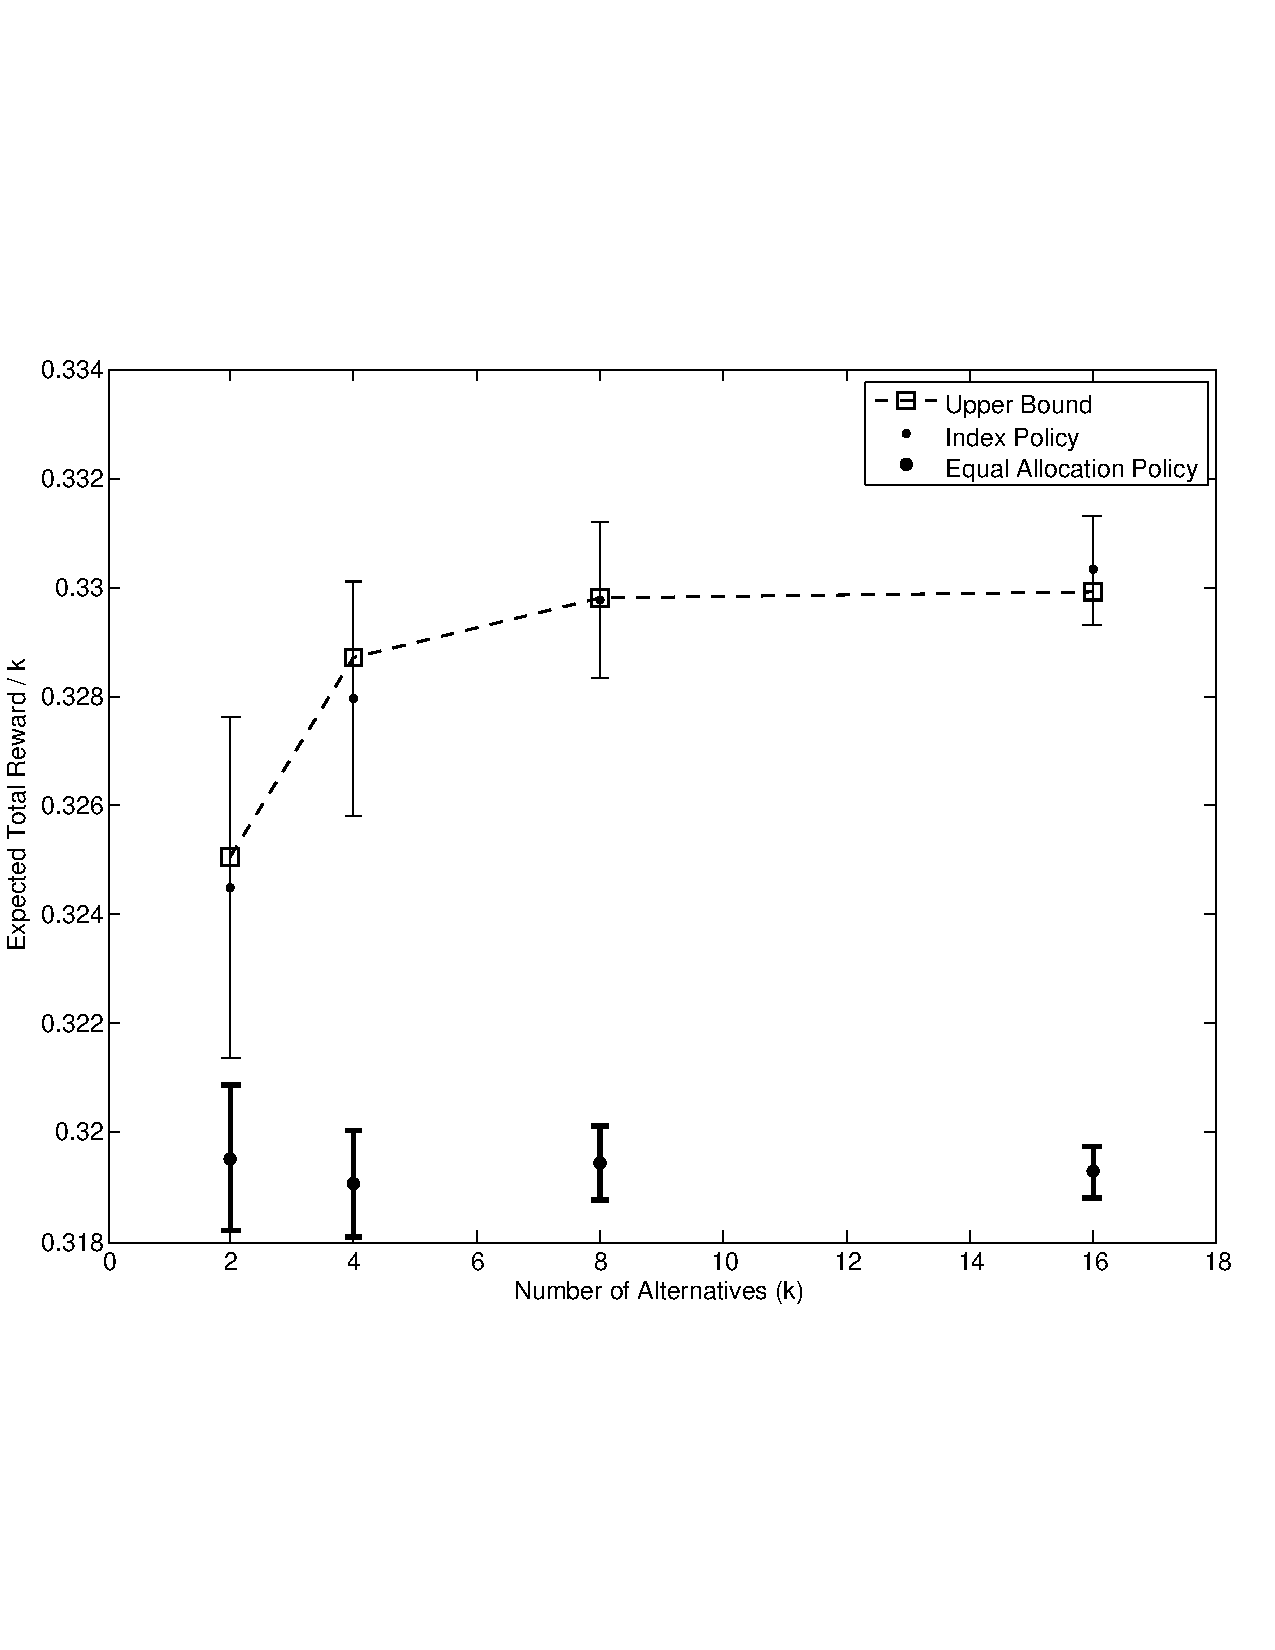
\includegraphics[width=9.7cm]{simPlots_0707_cropped.pdf}

\end{frame}
%%%%%%%%%%%%%%%%%%%%%%%%%%%%%%%%%%%%%%%%%%%%%%%

%%%%%%%%%%%%%%%%%%%%%%%%%%%%%%%%%%%%%%%%%%%%%%%
\begin{frame}{Numerical experiment}

For each $k=4,8,12, 16$
\begin{itemize}
\item $m = 1.25k$
\item $d_x = 0.5, \forall x \in \{1,...,k\}$
\item $(\alphav_0,\betav_0)=(1,1)^k$
\item $\square$ -- Upper bound
\item {\color{red}--} 95\% confidence interval with index policy, based on 10000 replications
\item {\huge\textbf{--}}  95\% confidence interval with equal allocation policy, based on 50000 replications
\item {\huge\textbf{- -}} 95\% confidence interval with optimistic knowledge gradient policy (Chen et al 2013), based on 10000 replications. 
\end{itemize}

\end{frame}
%%%%%%%%%%%%%%%%%%%%%%%%%%%%%%%%%%%%%%%%%%%%%%%


%%%%%%%%%%%%%%%%%%%%%%%%%%%%%%%%%%%%%%%%%%%%%%%
\begin{frame}{Numerical experiment}
%\centering
%\includegraphics[width=9.7cm]{plotSimUp_okg_cropped.pdf}

\end{frame}
%%%%%%%%%%%%%%%%%%%%%%%%%%%%%%%%%%%%%%%%%%%%%%%

%%%%%%%%%%%%%%%%%%%%%%%%%%%%%%%%%%%%%%%%%%%%%%%
\begin{frame}
\frametitle{Conjecture: Index policy is asymptotically optimal}
Conjecture: The index policy perform asymptotically close to an optimal policy as $k$ tends to infinity while keeping the number of resources to task ratio ($m/k$ or $N/k$) constant.
\end{frame}
%%%%%%%%%%%%%%%%%%%%%%%%%%%%%%%%%%%%%%%%%%%%%%%

%%%%%%%%%%%%%%%%%%%%%%%%%%%%%%%%%%%%%%%%%%%%%%%
\begin{frame}{Future Work}
\begin{itemize}
\item Prove the conjecture.
\item Conduct numerical experiment on a larger scale
\item Conduct experiment using index policy using Amazon Mechanic Turk in real time.
\item Apply the same method to ranking $\&$ selection problems.
\end{itemize}
\end{frame}
%%%%%%%%%%%%%%%%%%%%%%%%%%%%%%%%%%%%%%%%%%%%%%%

%%%%%%%%%%%%%%%%%%%%%%%%%%%%%%%%%%%%%%%%%%%%%%%
\begin{frame}
\frametitle{Publication strategy}
\begin{itemize}
\item Accepted: "Parallel Bayesian policy for finite-horizon
multiple comparisons with a known standard". Proceedings of the 2014 Winter Simulation Conference 2014.
\item Rejected: "Bayes-Optimal Effort Allocation in Crowdsourcing: Bounds and Index Policies", ICML 2015.
\end{itemize}
\end{frame}
%%%%%%%%%%%%%%%%%%%%%%%%%%%%%%%%%%%%%%%%%%%%%%%

%%%%%%%%%%%%%%%%%%%%%%%%%%%%%%%%%%%%%%%%%%%%%%%%
\begin{frame}
\centering
{\Huge Thank you!}
\end{frame}

\end{document}










